\chapter{Results and Evaluation}
\label{ch:results}
\label{sec:results_and_evaluation}

\section{Empirical Parameter Verification}
To instantiate the theoretical models derived in Chapter~\ref{ch:design_methodology}, we first characterize the system parameters experimentally. This includes measuring the computational overhead ($t_{ver}$) and calculating the theoretical collision probabilities ($p_{miss}$).

\subsection{Encoding Latency ($t_{ver}$)}
The computational overhead of the encoding step, $t_{ver}$, was measured empirically by running 100{,}000 \texttt{send} operations for each system configuration. In addition to the sample mean, we estimate a \textbf{95\% confidence interval (CI)} for the mean using a batch timing method (100 timing batches, each covering an equal share of operations).

\textbf{Interpretation of Table~\ref{tab:tver_results_bits}:}
The table reports the \emph{sample mean} $\bar{t}_{ver}$ in microseconds. The CI quantifies measurement uncertainty due to runtime noise (OS scheduling, cache effects, Python overhead). In our measurements, the 95\% CI half-widths are below \textbf{1\,$\mu s$} for all configurations. Therefore, the reported means are sufficiently stable for the latency-model comparisons in this chapter.

Note that the \textbf{mean} values can shift slightly across runs and machines (Python runtime, CPU frequency scaling, background load). For reproducibility and consistency with the figures in this chapter, we keep the table mean values aligned with the parameter set used for the plotted latency evaluation, and we report representative 95\% CI half-widths to quantify the measurement uncertainty.

\begin{table}[!htbp]  % Prefer LaTeX float placement (float package not required)
    \centering
    \caption{Measured Verification Time $t_{ver}$ (mean $\pm$ 95\% CI half-width, with relative half-width)}
    \label{tab:tver_results_bits}
    \begin{tabular}{lrr}
        \toprule
        & \multicolumn{2}{c}{$n_{ver}$ (bits)} \\
        \cmidrule(lr){2-3}
        System ($n_{data}$) & 4 & 16 \\
        \midrule
        \textbf{SHA-256} & & \\
        96 bits & $2.13\pm0.04\,(1.9\%)$ & $2.24\pm0.01\,(0.4\%)$ \\
        4001 bits & $14.65\pm0.31\,(2.1\%)$ & $15.41\pm0.09\,(0.6\%)$ \\
        \midrule
        \textbf{RS-ID} & & \\
        96 bits & $14.55\pm0.39\,(2.7\%)$ & $3.79\pm0.02\,(0.5\%)$ \\
        4001 bits & $51.78\pm0.94\,(1.8\%)$ & $38.57\pm0.36\,(0.9\%)$ \\
        \bottomrule
    \end{tabular}
\end{table}

\textbf{Analysis of $t_{ver}$ Results:}
The measurement results in Table~\ref{tab:tver_results_bits} reveal distinct performance characteristics between the algebraic (RS-ID) and cryptographic (SHA-256) approaches:

\begin{enumerate}
    \item \textbf{Stability of SHA-256:} Consistent with the theoretical discussion in Section~\ref{sec:reliability_analysis}, the computation time of SHA-256 is largely insensitive to the output verifier length. For the short payload ($n_{data}=96$ bits), the latency remains nearly constant (\textasciitilde 2.2~$\mu s$) when truncating to either $n_{ver}=4$ or $n_{ver}=16$ bits. When increasing the payload to $n_{data}=4001$ bits, the latency rises to \textasciitilde 15~$\mu s$, which is expected due to the block-based processing of SHA.
    
    \item \textbf{The Chunking Effect in RS-ID:} A counter-intuitive phenomenon is observed for RS-ID: for the small payload ($n_{data}=96$ bits), increasing the verifier length from $n_{ver}=4$ to $n_{ver}=16$ bits \textit{reduces} the measured latency substantially (from 14.55~$\mu s$ to 3.79~$\mu s$).
    This can be explained by the polynomial construction mechanism. RS-ID represents the input as $k$ coefficients, where $k=\lceil n_{data}/n_{ver} \rceil$. With $n_{ver}=4$, the data is sliced into 24 chunks, requiring more iterations of field operations. With $n_{ver}=16$, the chunk count drops to 6. For small datasets, the reduction in loop iterations outweighs the increased per-operation cost of arithmetic in a larger field.
\end{enumerate}

\subsection{Theoretical Collision Probability ($p_{miss}$)}
Based on the bounds derived in Chapter~\ref{ch:design_methodology} (Equations~\eqref{eq:sha_bound} and~\eqref{eq:rsid_bound}), we compute the theoretical collision probability $p_{miss}$ for the parameter grid used in the latency model. Note that for RS-ID, if the polynomial degree exceeds the field size, the bound is capped at 1.0.

\begin{table}[!htbp] % Prefer LaTeX float placement (float package not required)
    \centering
    \caption{Theoretical Collision Probability ($p_{miss}$) for Bit-Based Parameters}
    \label{tab:pmiss_results_bits}
    \begin{tabular}{lrr}
        \toprule
        & \multicolumn{2}{c}{$n_{ver}$ (bits)} \\
        \cmidrule(lr){2-3}
        System ($n_{data}$) & 4 & 16 \\
        \midrule
        \textbf{SHA-256 (any $n_{data}$)} & $6.25\times 10^{-2}$ & $1.53\times 10^{-5}$ \\
        \midrule
        \textbf{RS-ID} & & \\
        96 bits & $1.00$ & $9.16\times 10^{-5}$ \\
        4001 bits & $1.00$ & $3.83\times 10^{-3}$ \\
        \bottomrule
    \end{tabular}
\end{table}

\section{End-to-End Latency Evaluation}
Using the hybrid latency model and the calibrated parameters from Section 5.1, we analyze the system performance across varying network conditions and prediction qualities.

\subsection{Sensitivity to Channel Bandwidth}
We first evaluate the expected latency as a function of channel bandwidth ($B$). Figures~\ref{fig:latency_vs_bandwidth_96bits} and~\ref{fig:latency_vs_bandwidth_4001bits} compare the Traditional approach against the ID-based schemes.

\begin{figure}[!htbp]
    \centering
    \begin{minipage}[t]{0.49\textwidth}
        \centering
        
\includegraphics[width=\linewidth]{figures/plots/latency_empirical_bandwidth_96bits.png}
        \captionof{figure}{Expected latency vs. bandwidth for $n_{data}=96$ bits ($p_{desync}=0.1$).}
        \label{fig:latency_vs_bandwidth_96bits}
    \end{minipage}\hfill
    \begin{minipage}[t]{0.49\textwidth}
        \centering
        
\includegraphics[width=\linewidth]{figures/plots/latency_empirical_bandwidth_4001bits.png}
        \captionof{figure}{Expected latency vs. bandwidth for $n_{data}=4001$ bits ($p_{desync}=0.1$).}
        \label{fig:latency_vs_bandwidth_4001bits}
    \end{minipage}
\end{figure}

\textbf{Discussion (Bandwidth Trade-off):}
The results illustrate the dominance of the Identification scheme in bandwidth-constrained environments. 
\begin{itemize}
    \item \textbf{Low Bandwidth Regime ($B < 1$ Mbps):} The transmission time of raw data dominates the Traditional latency. The ID scheme offers an order-of-magnitude reduction by transmitting only the compact verifier.
    \item \textbf{High Bandwidth Regime ($B > 10$ Mbps):} As transmission becomes instantaneous, the latency floor is determined by the computational overhead $t_{ver}$. Consequently, the Traditional scheme (which has zero encoding overhead) eventually outperforms the ID schemes, creating a clear "Cross-over Point."
\end{itemize}

\subsection{Sensitivity to Prediction Quality}
Next, we examine the impact of the Digital Twin's prediction accuracy ($p_{desync}$) at a fixed bandwidth ($B=5$ Mbps).

\begin{figure}[!htbp]
    \centering
    \begin{minipage}[t]{0.49\textwidth}
        \centering
        
\includegraphics[width=\linewidth]{figures/plots/latency_vs_desync_96bits.png}
        \captionof{figure}{Expected latency vs. $p_{desync}$ for $n_{data}=96$ bits ($B=5$ Mbps).}
        \label{fig:latency_vs_desync_96bits}
    \end{minipage}\hfill
    \begin{minipage}[t]{0.49\textwidth}
        \centering
        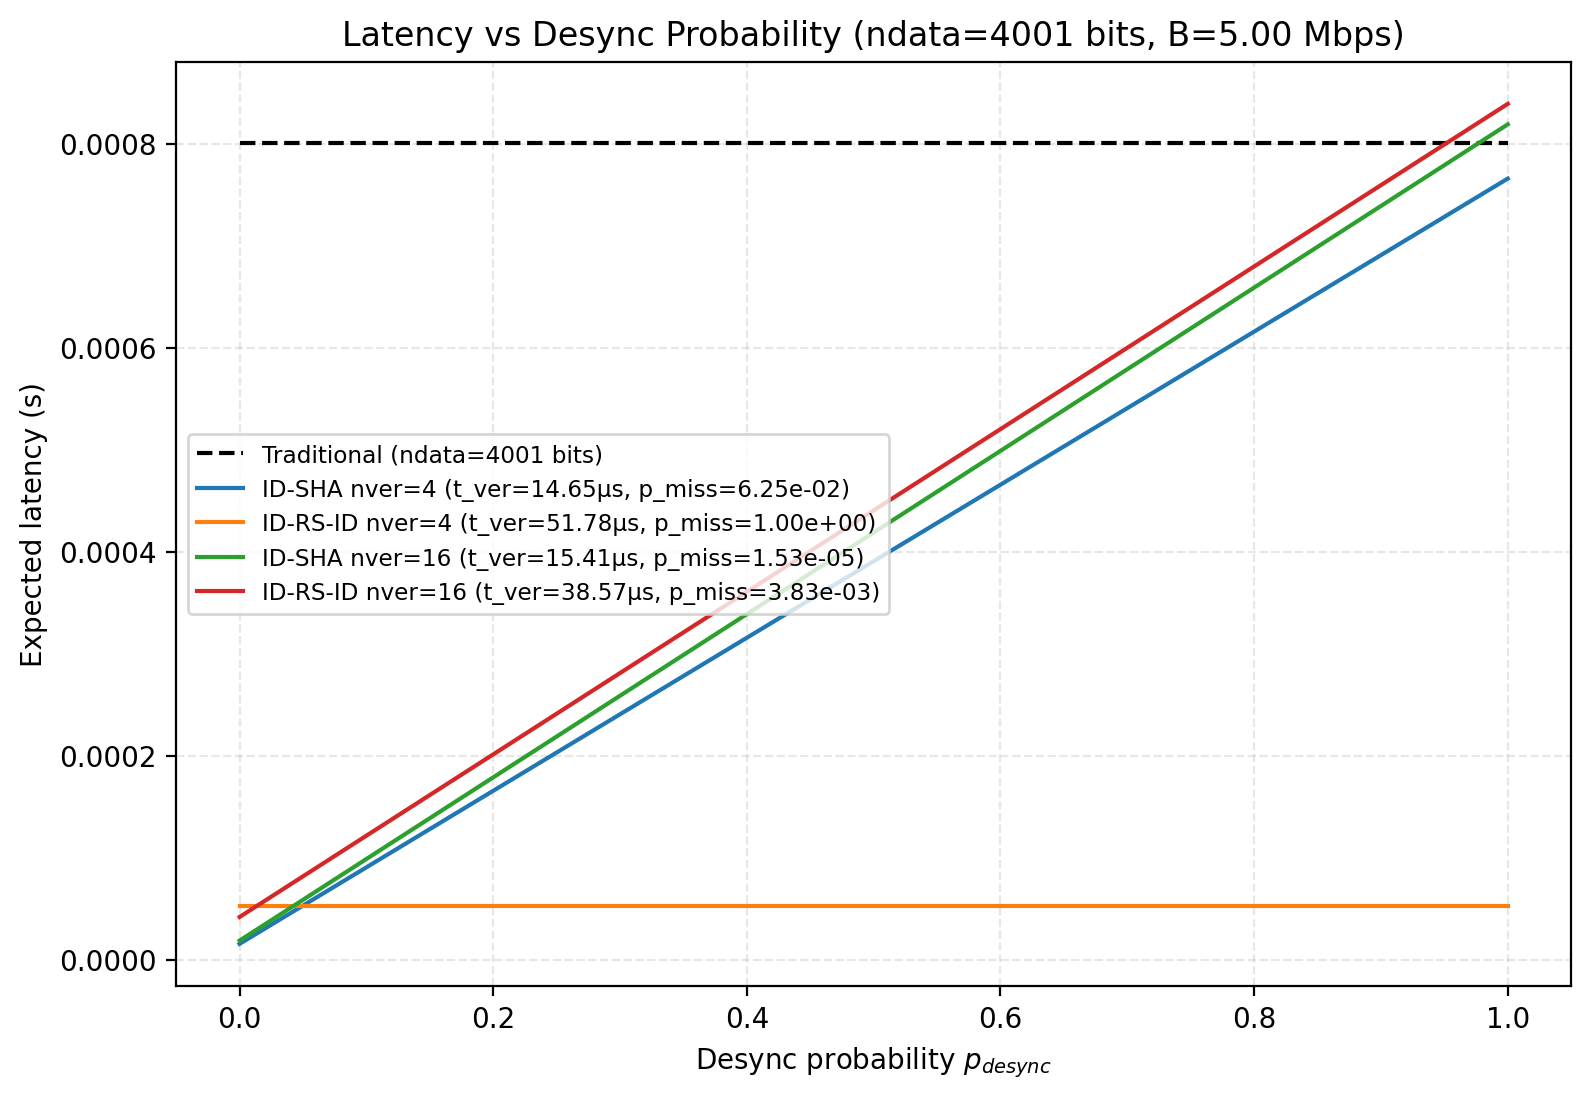
\includegraphics[width=\linewidth]{figures/plots/latency_vs_desync_4001bits.png}
        \captionof{figure}{Expected latency vs. $p_{desync}$ for $n_{data}=4001$ bits ($B=5$ Mbps).}
        \label{fig:latency_vs_desync_4001bits}
    \end{minipage}
\end{figure}

\textbf{Discussion (Prediction Quality):}
\begin{itemize}
    \item \textbf{Break-even Analysis:} For the short payload (Fig.~\ref{fig:latency_vs_desync_96bits}), the ID-SHA curves intersect the Traditional line at approximately $p_{desync} \approx 0.8$. This implies that ID is beneficial as long as the Digital Twin's prediction accuracy exceeds 20\%. For the large payload (Fig.~\ref{fig:latency_vs_desync_4001bits}), the transmission penalty is so high that ID-SHA remains superior across nearly the entire range of $p_{desync}$.
    
    \item \textbf{Anomaly Analysis (RS-ID $n_{ver}=4$):} 
    A notable anomaly appears in the RS-ID results for $n_{ver}=4$ bits (orange line in Fig.~\ref{fig:latency_vs_desync_96bits}), which appears flat and low. This is a \textbf{theoretical artifact} caused by the saturation of collision probability ($p_{miss}=1.0$, see Table~\ref{tab:pmiss_results_bits}). Mathematically, this sets the fallback penalty term to zero. In reality, this represents a catastrophic failure where desynchronization is never detected. Therefore, this configuration is invalid for safety-critical systems despite its apparent low latency.
\end{itemize}

\section{K-ID Safety--Latency Trade-off}
\label{sec:kid_results}
This section evaluates the tolerance-based K-ID model introduced in Section~\ref{sec:kid_model} and implemented as described in Section~\ref{sec:kid_setup}. The experiment sweeps $n_{ver}\in\{4,8,12,16\}$ and $K\in\{2,5,10,20\}$ for a 96-bit payload at $B=1$ Mbps.

\subsection{Sweep Results}
Figure~\ref{fig:kid_sweep_overview} summarizes the main metrics. The miss rate is plotted as the conditional safety risk $\Pr[\mathrm{accept}\mid\mathrm{unsafe}]$, i.e., the probability that an unsafe state is incorrectly accepted due to a verifier collision with the acceptable set.

\begin{figure}[!htbp]
    \centering
    \begin{subfigure}[t]{0.49\textwidth}
        \centering
        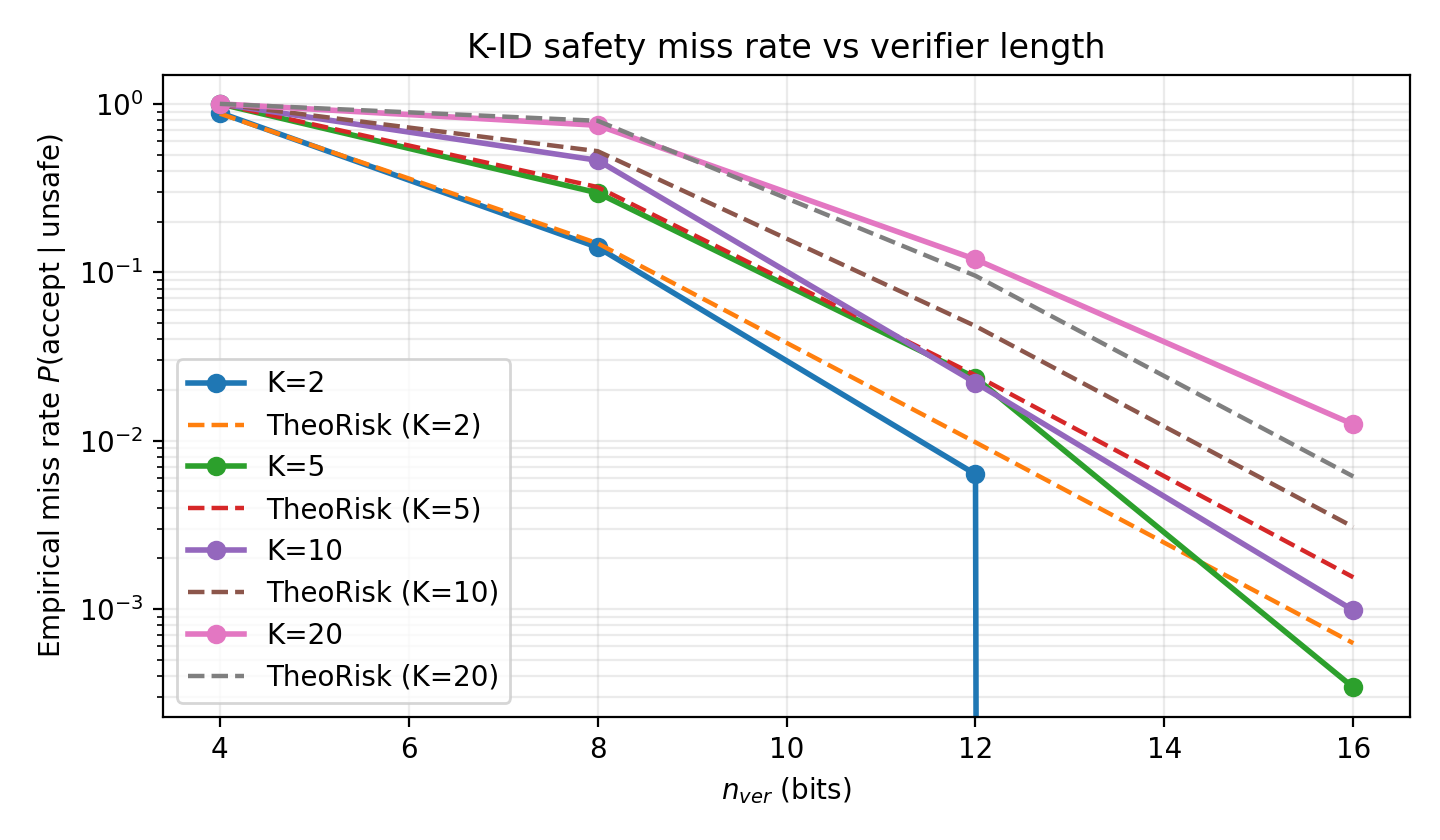
\includegraphics[width=\linewidth]{figures/plots/kid_sweep_miss_rate.png}
        \caption{Conditional miss rate $\Pr[\mathrm{accept}\mid\mathrm{unsafe}]$.}
        \label{fig:kid_miss_rate}
    \end{subfigure}\hfill
    \begin{subfigure}[t]{0.49\textwidth}
        \centering
        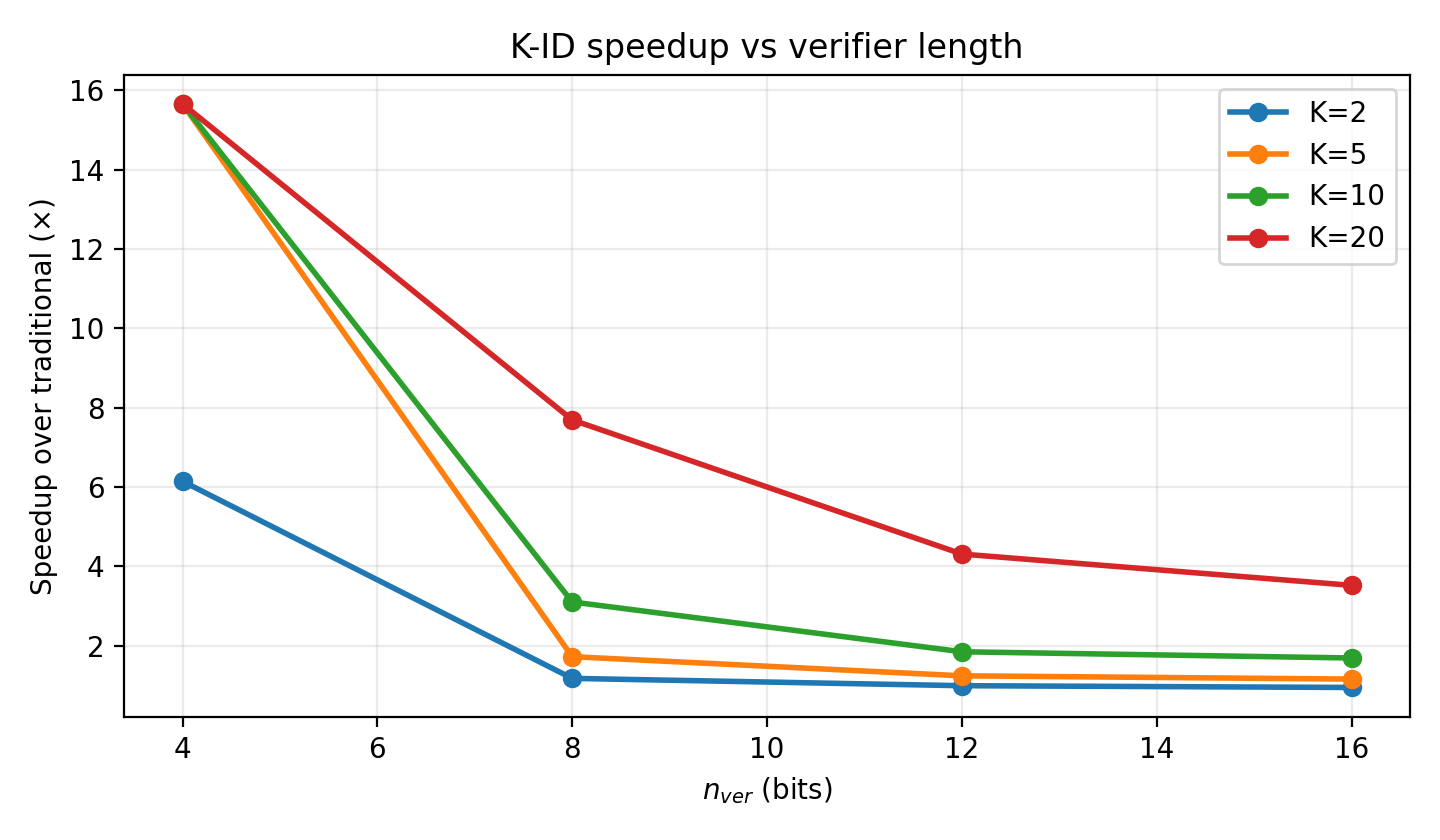
\includegraphics[width=\linewidth]{figures/plots/kid_sweep_speedup.png}
        \caption{Speedup over traditional transmission.}
        \label{fig:kid_speedup}
    \end{subfigure}

    \vspace{0.6em}

    \begin{subfigure}[t]{0.49\textwidth}
        \centering
        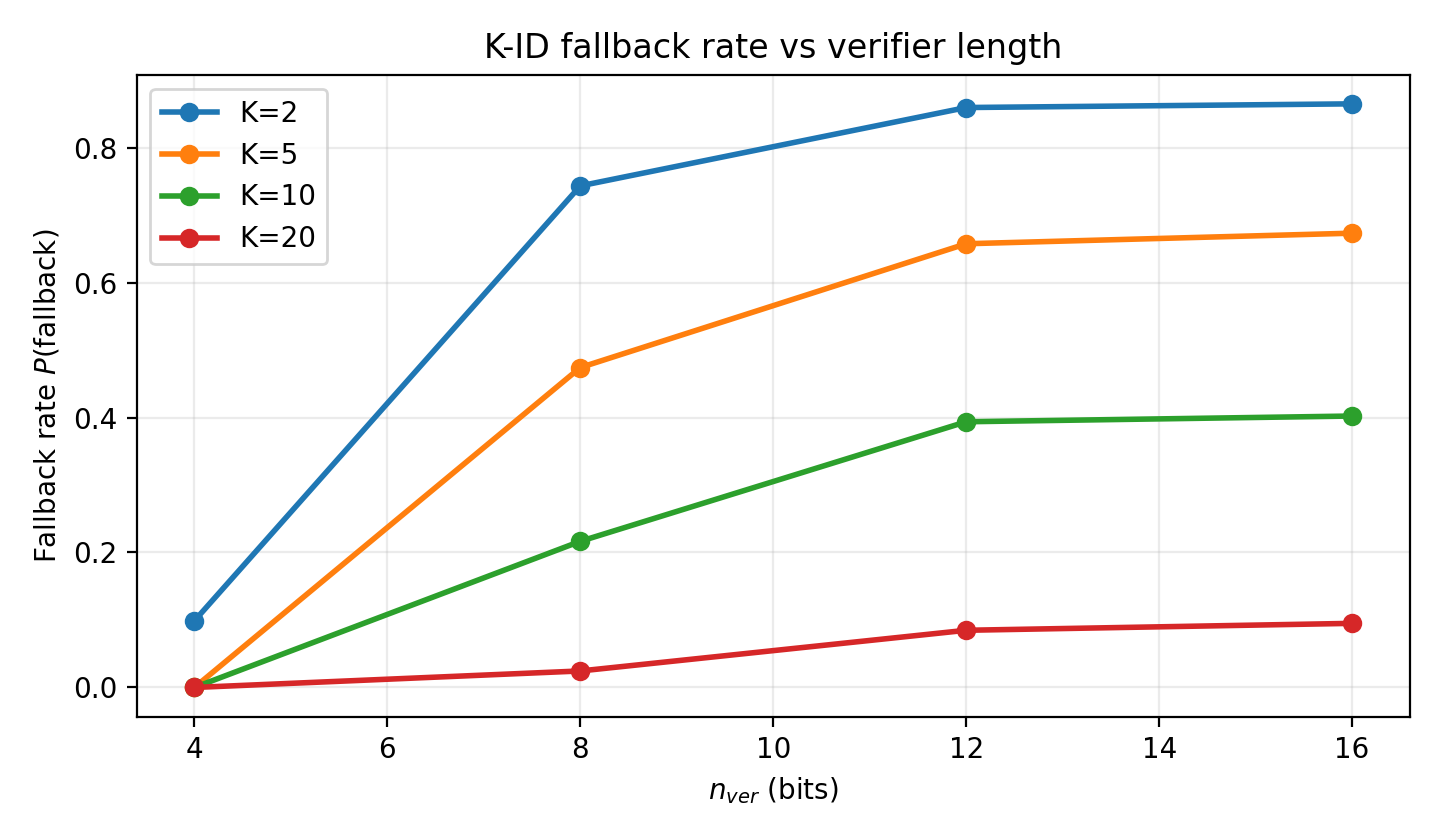
\includegraphics[width=\linewidth]{figures/plots/kid_sweep_fallback_rate.png}
        \caption{Fallback probability $\Pr[\mathrm{fallback}]$.}
        \label{fig:kid_fallback_rate}
    \end{subfigure}\hfill
    \begin{subfigure}[t]{0.49\textwidth}
        \centering
        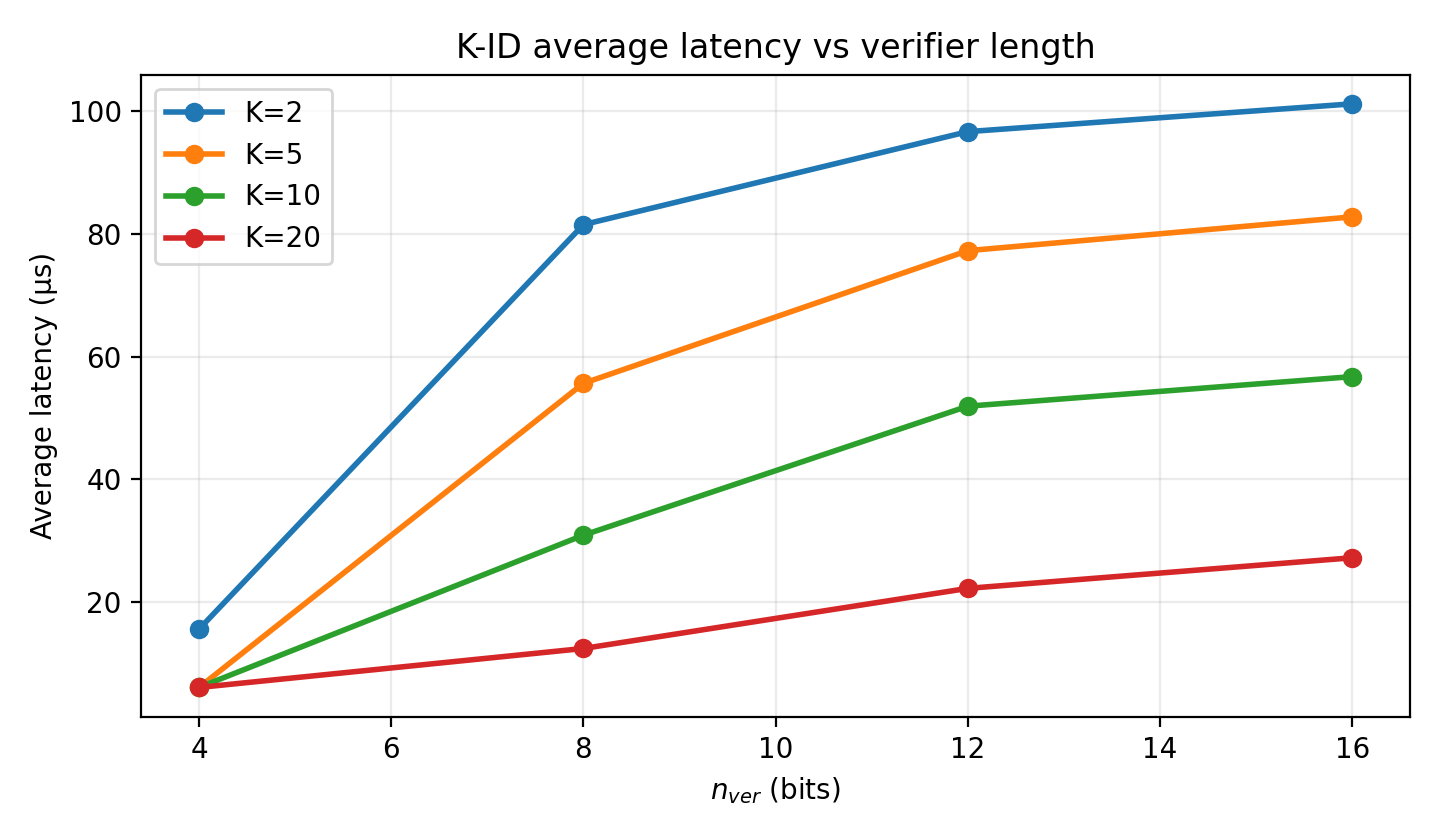
\includegraphics[width=\linewidth]{figures/plots/kid_sweep_latency.png}
        \caption{Expected latency under Equation~\eqref{eq:kid_latency}.}
        \label{fig:kid_latency}
    \end{subfigure}

    \caption{K-ID parameter sweep results for $n_{data}=96$ bits at $B=1$ Mbps.}
    \label{fig:kid_sweep_overview}
\end{figure}

\textbf{Analysis (Effect of $n_{ver}$):}
Increasing $n_{ver}$ reduces the conditional miss rate approximately exponentially, consistent with the Random Oracle scaling in Equation~\eqref{eq:kid_sha_bound}. However, a larger $n_{ver}$ also increases the mandatory verifier transmission term $n_{ver}/B$ and, more importantly, reduces the chance of ``accidental acceptance'' when unsafe, which increases detection and therefore increases fallback frequency. As a result, higher $n_{ver}$ improves safety but can reduce speedup (and increase latency) depending on how often the system enters unsafe states.

\textbf{Analysis (Effect of $K$):}
Increasing $K$ enlarges the acceptable set. This has two opposing effects that are visible in Figure~\ref{fig:kid_sweep_overview}:
\begin{itemize}
    \item The conditional miss rate $\Pr[\mathrm{accept}\mid\mathrm{unsafe}]$ increases with $K$, because more acceptable states mean more opportunities for a hash collision with an unsafe verifier.
    \item The fallback rate and latency decrease with $K$ because the system is unsafe less often (fewer ticks lie outside the tolerance interval), so the expensive full-payload fallback is triggered less frequently.
\end{itemize}
This demonstrates the fundamental K-ID trade-off: a larger tolerance improves performance and reduces fallback, but raises the conditional risk of accepting an unsafe state.

\subsection{Pareto Frontier Interpretation}
To make the trade-off explicit, Figure~\ref{fig:kid_pareto} plots speedup against the \emph{conditional} miss rate $P(\mathrm{accept}\mid\mathrm{unsafe})$ and highlights the non-dominated (Pareto-optimal) configurations.

\begin{figure}[!htbp]
    \centering
    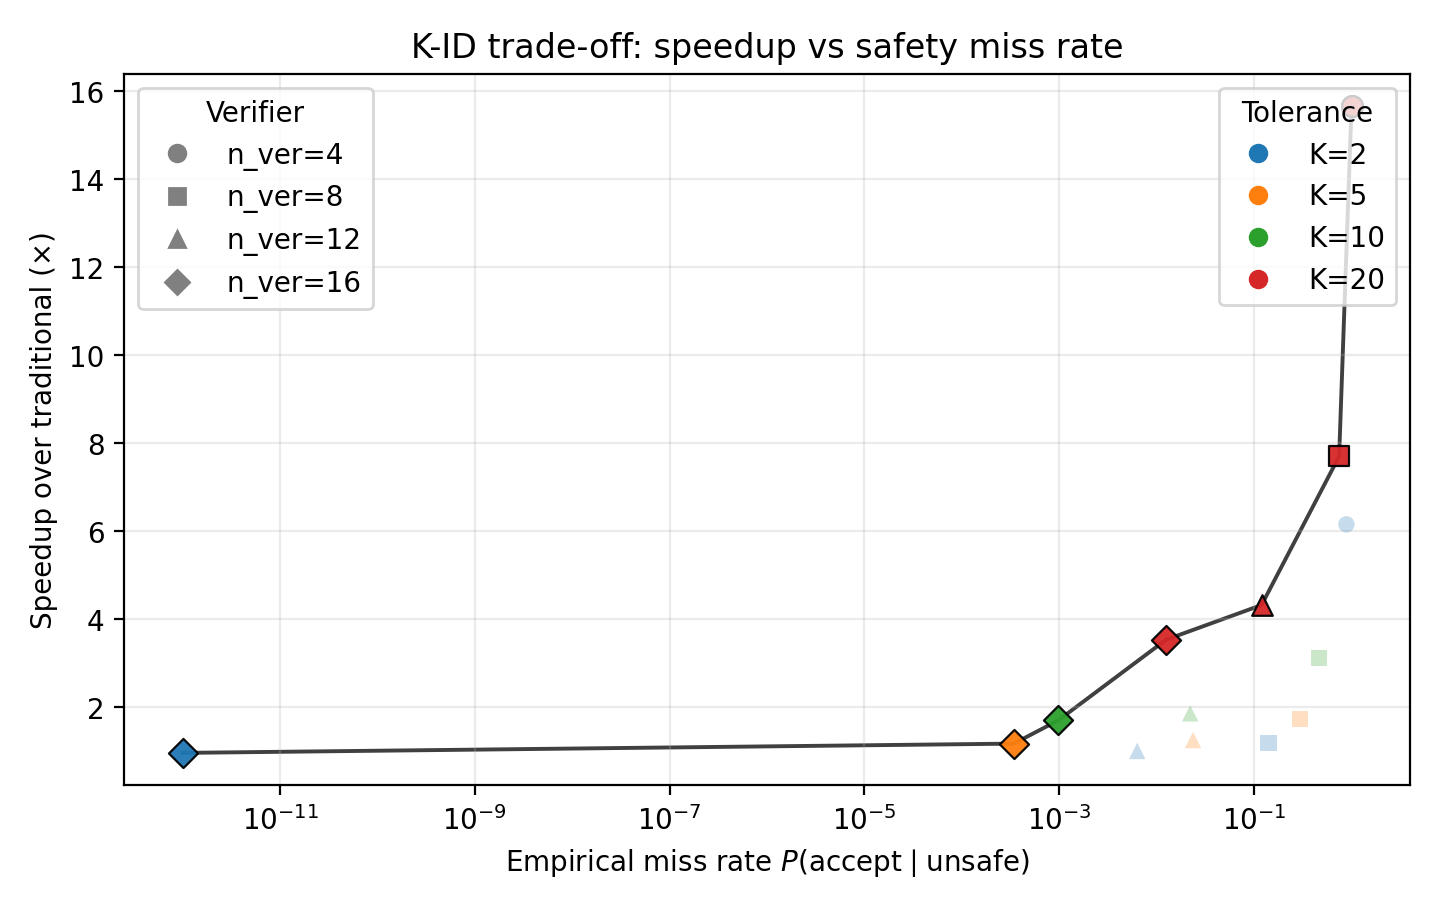
\includegraphics[width=0.72\textwidth]{figures/plots/kid_sweep_pareto.png}
    \caption{Pareto view of the K-ID trade-off: speedup vs. conditional miss rate $P(\mathrm{accept}\mid\mathrm{unsafe})$.}
    \label{fig:kid_pareto}
\end{figure}

\textbf{Overall Risk vs. Conditional Miss Rate:}
The x-axis in Figure~\ref{fig:kid_pareto} is a \emph{conditional} safety metric: it describes how likely an unsafe state is accepted \emph{given that} the system is already unsafe. To assess end-to-end operational risk, it is often more informative to consider the \emph{overall} probability of an unsafe acceptance per tick,
\begin{equation}
    P(\mathrm{unsafe}\cap\mathrm{accept}) = P(\mathrm{unsafe})\cdot P(\mathrm{accept}\mid\mathrm{unsafe}).
\end{equation}
This overall risk accounts for how frequently unsafe states occur (which depends strongly on $K$ and the prediction error distribution). Figure~\ref{fig:kid_pareto_overall} therefore replots the trade-off using $P(\mathrm{unsafe}\cap\mathrm{accept})$ on the x-axis.

\begin{figure}[!htbp]
    \centering
    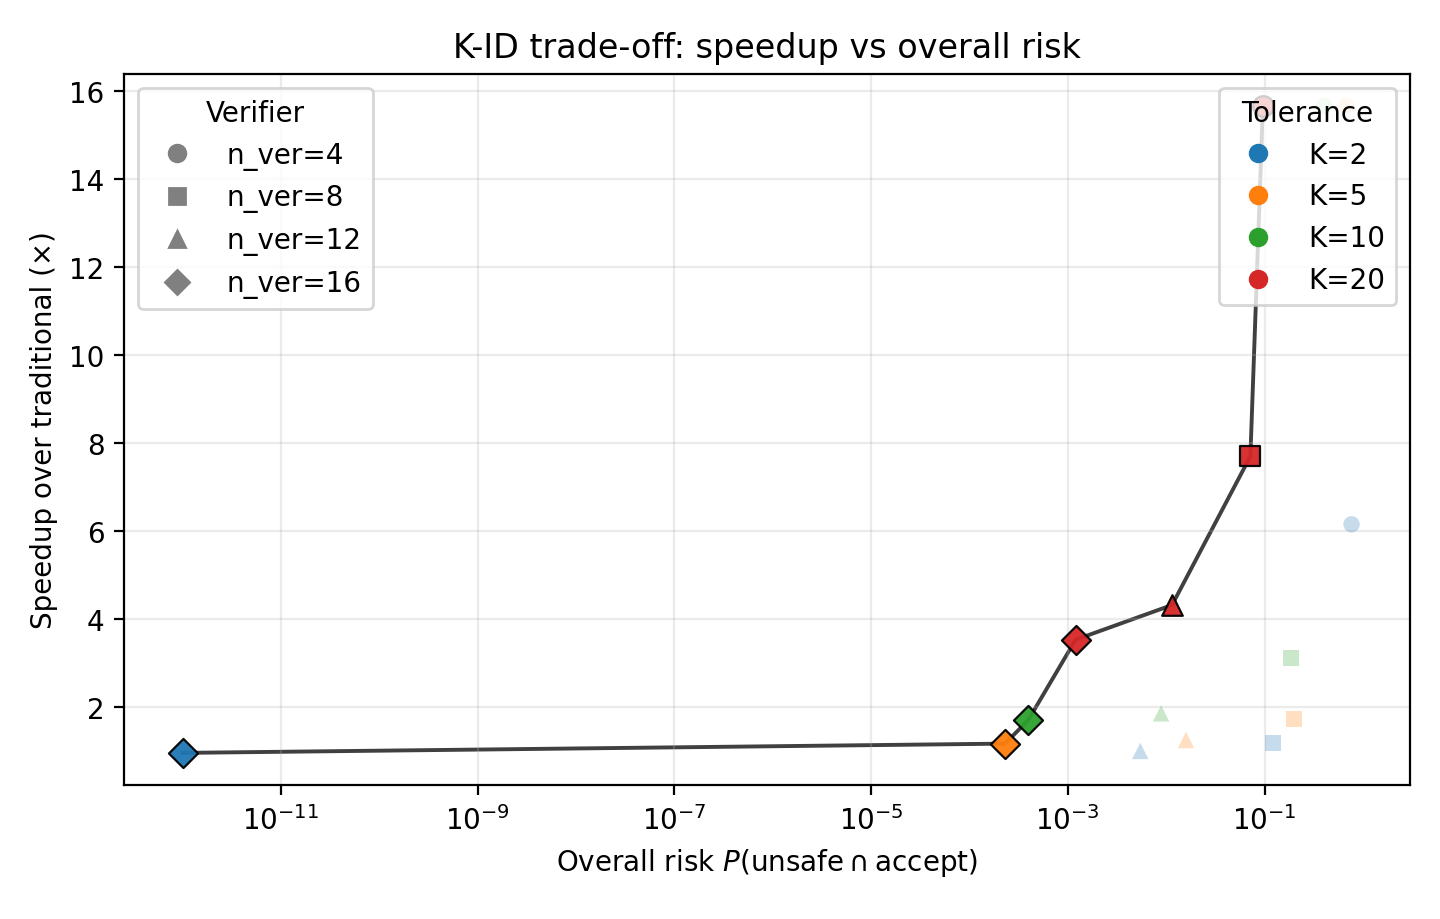
\includegraphics[width=0.72\textwidth]{figures/plots/kid_sweep_pareto_overall_risk.png}
    \caption{Pareto view using overall risk $P(\mathrm{unsafe}\cap\mathrm{accept})$: speedup vs. total unsafe-accept probability per tick.}
    \label{fig:kid_pareto_overall}
\end{figure}

\textbf{Discussion:}
The solid curve in Figure~\ref{fig:kid_pareto} connects the Pareto-optimal configurations (the \emph{frontier}). These points represent operating choices where improving safety (moving left, lower conditional miss rate) necessarily requires sacrificing speedup (moving down), and vice versa. Points in the lower-right region are \emph{dominated} (simultaneously slower and less safe) and can be discarded.

In deployment, the choice of $(K,n_{ver})$ should be driven by an application-level safety budget on $p_{miss,K}$ (or an overall risk measure that also weights the unsafe frequency) together with a latency target. The sweep provides a practical menu of operating points to select from based on these constraints.

\subsection{RS-ID Comparison and Uniform Error Model}
The baseline K-ID sweep above uses a truncated SHA-256 verifier and a Gaussian prediction error. To compare against the algebraic verifier family, we rerun the sweep with an \textbf{RS-ID} verifier (single-tag, tag position 2) and replace the error model with a \textbf{uniform} distribution centered at the mean. The uniform half-width is chosen to match the variance of the Gaussian case ($a=\sqrt{3}\,\sigma$).

Figure~\ref{fig:kid_uniform_compare} shows the resulting metrics side-by-side for \texttt{sha256\_trunc} and \texttt{rsid}. The overall trends remain consistent with the K-ID model: increasing $n_{ver}$ reduces collision-driven acceptance, while increasing $K$ reduces fallback frequency (by making unsafe states rarer), at the cost of enlarging the acceptable set.

\begin{figure}[!htbp]
    \centering
    \begin{subfigure}[t]{0.49\textwidth}
        \centering
        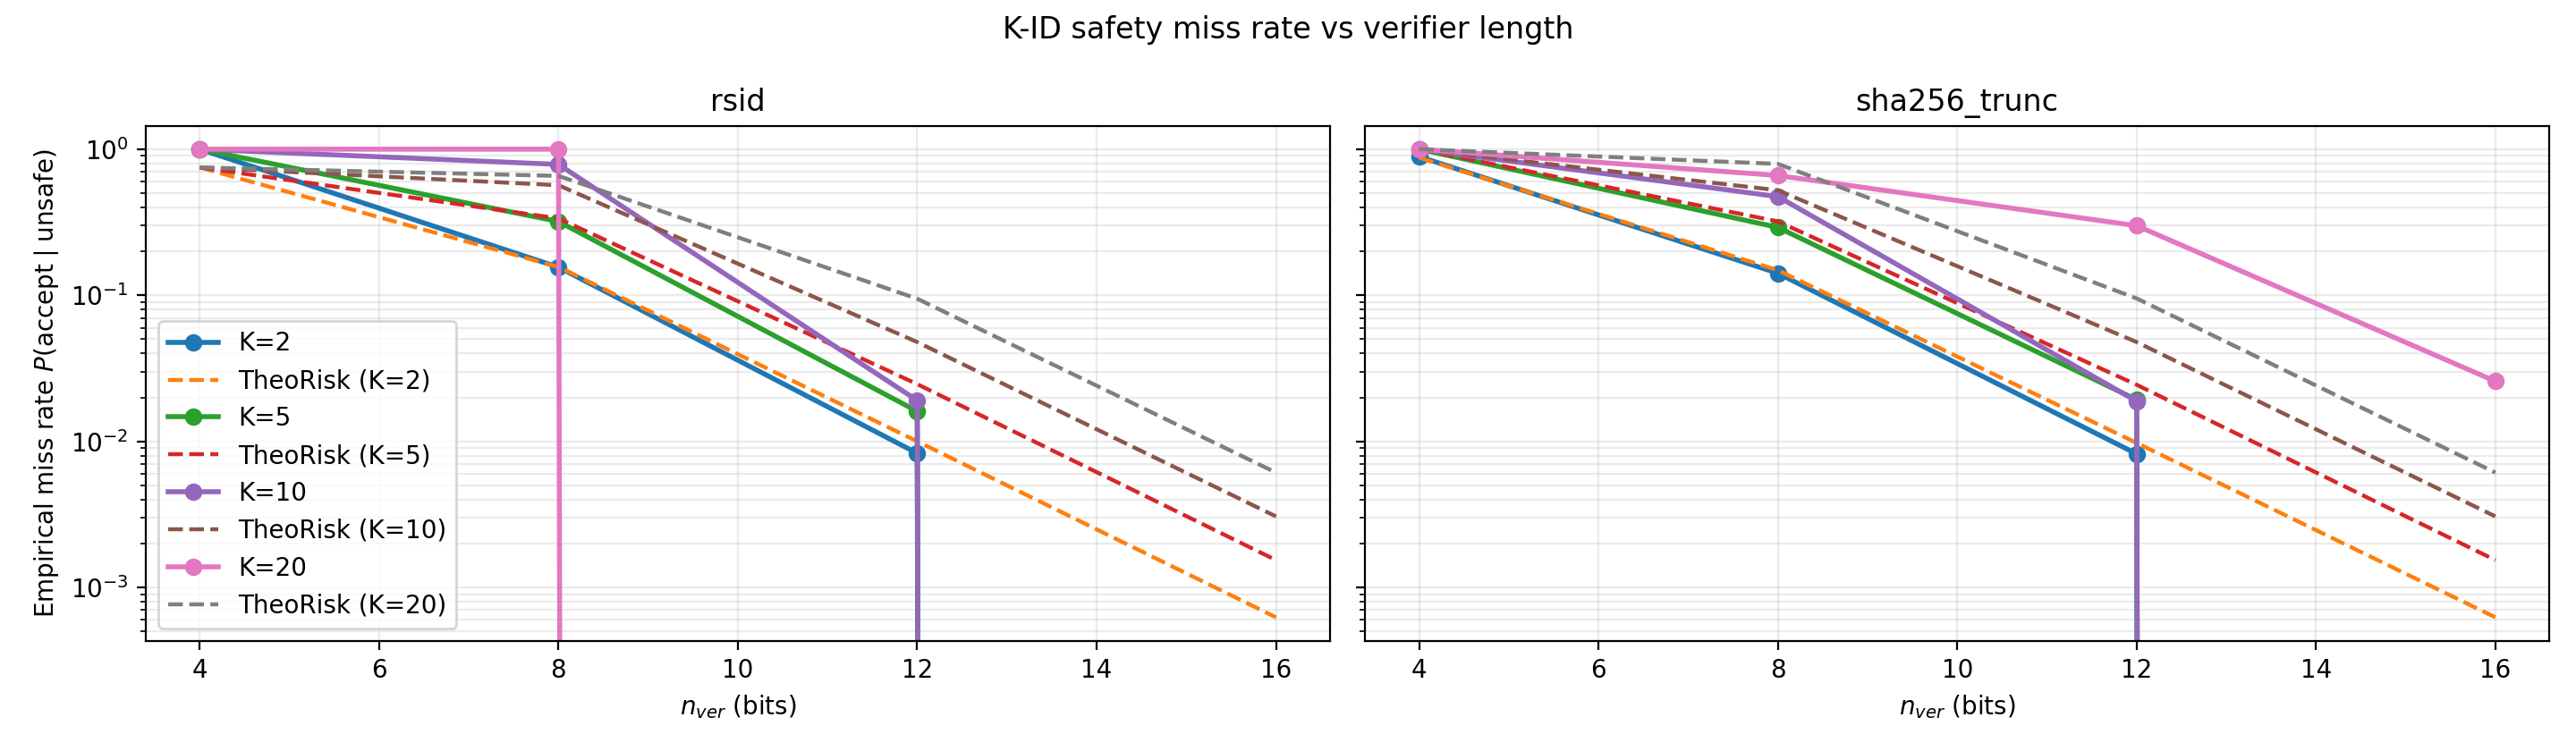
\includegraphics[width=\linewidth]{figures/plots/kid_sweep_uniform_both_miss_rate.png}
        \caption{Conditional miss rate (uniform error), by system.}
        \label{fig:kid_uniform_miss}
    \end{subfigure}\hfill
    \begin{subfigure}[t]{0.49\textwidth}
        \centering
        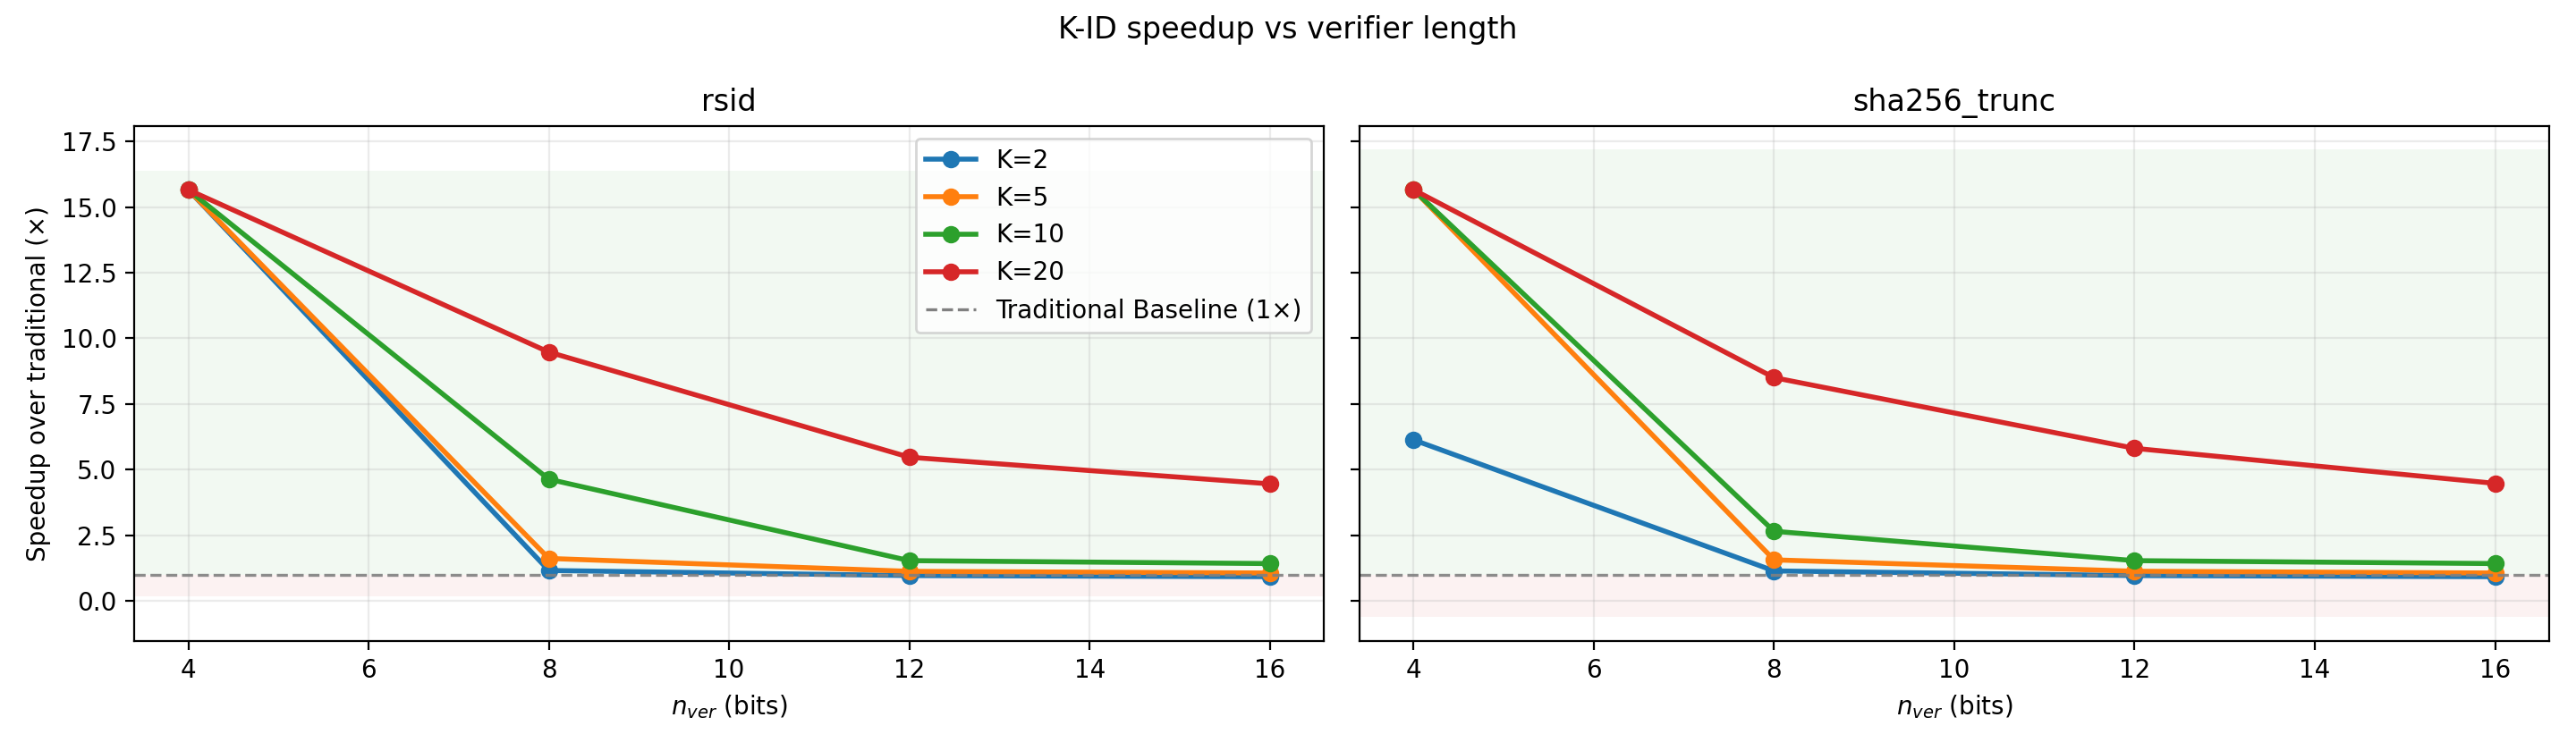
\includegraphics[width=\linewidth]{figures/plots/kid_sweep_uniform_both_speedup.png}
        \caption{Speedup (uniform error), by system.}
        \label{fig:kid_uniform_speedup}
    \end{subfigure}

    \vspace{0.6em}

    \begin{subfigure}[t]{0.49\textwidth}
        \centering
        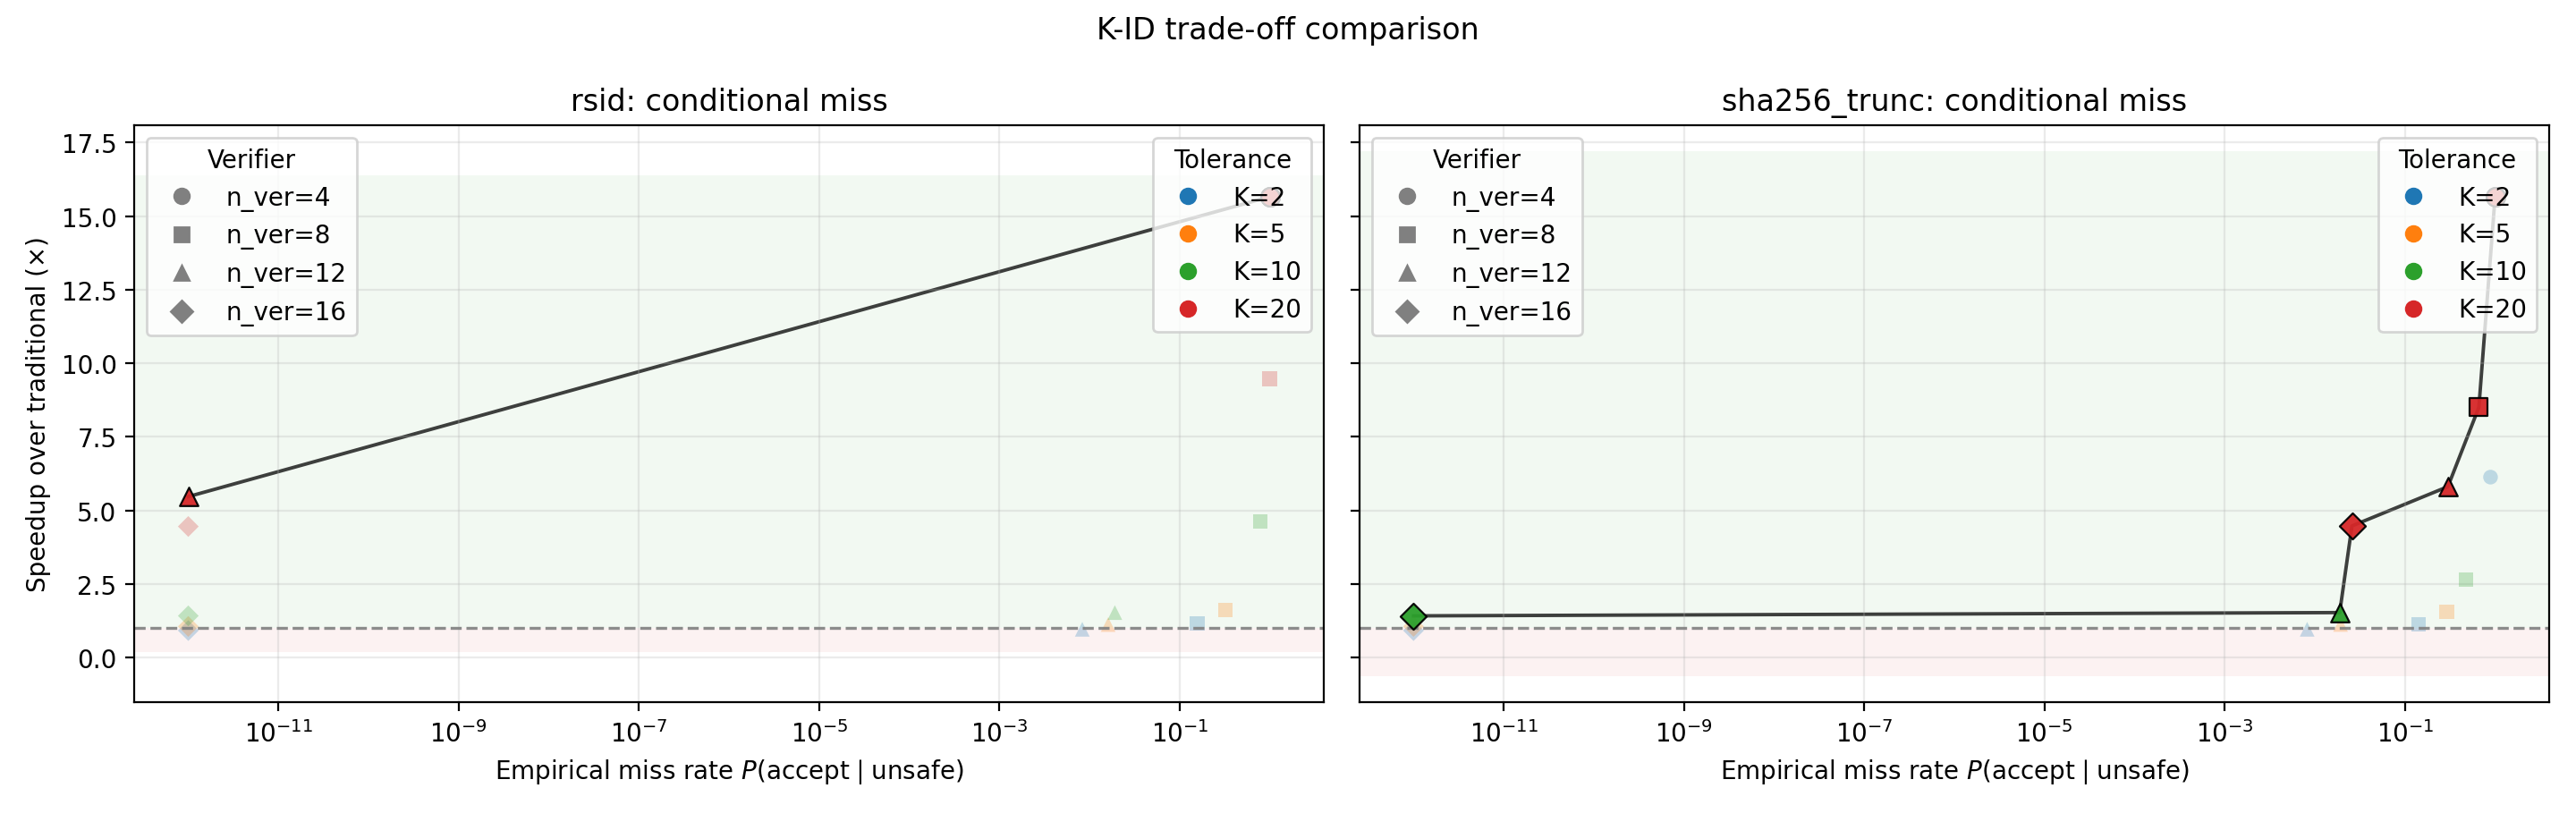
\includegraphics[width=\linewidth]{figures/plots/kid_sweep_uniform_both_pareto.png}
        \caption{Pareto trade-off: speedup vs. $P(\mathrm{accept}\mid\mathrm{unsafe})$.}
        \label{fig:kid_uniform_pareto}
    \end{subfigure}\hfill
    \begin{subfigure}[t]{0.49\textwidth}
        \centering
        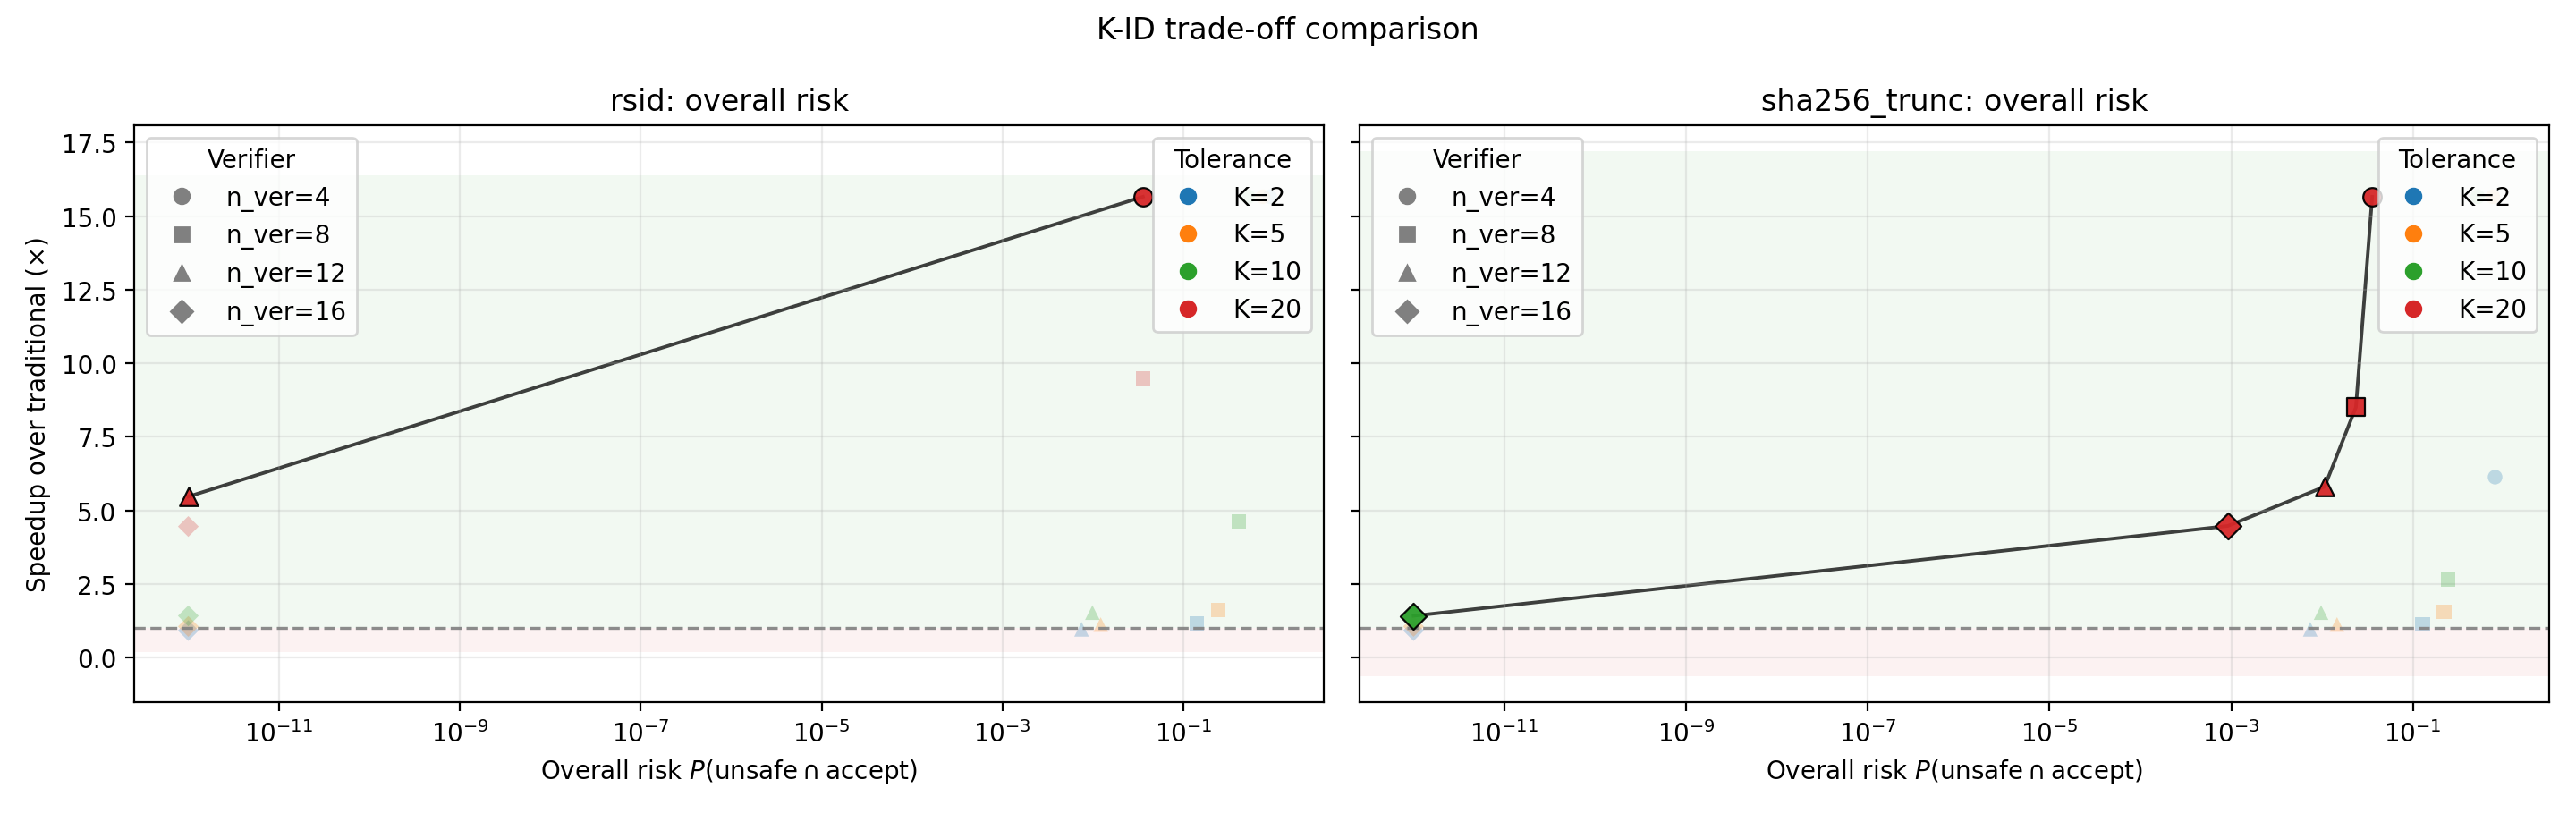
\includegraphics[width=\linewidth]{figures/plots/kid_sweep_uniform_both_pareto_overall_risk.png}
        \caption{Pareto trade-off: speedup vs. $P(\mathrm{unsafe}\cap\mathrm{accept})$.}
        \label{fig:kid_uniform_pareto_overall}
    \end{subfigure}

    \caption{K-ID sweep comparison of truncated SHA-256 vs. RS-ID under a uniform prediction error model ($n_{data}=96$ bits, $B=1$ Mbps).}
    \label{fig:kid_uniform_compare}
\end{figure}